\documentclass{standalone}
\usepackage{tikz}
\usetikzlibrary{patterns, positioning}


\begin{document}
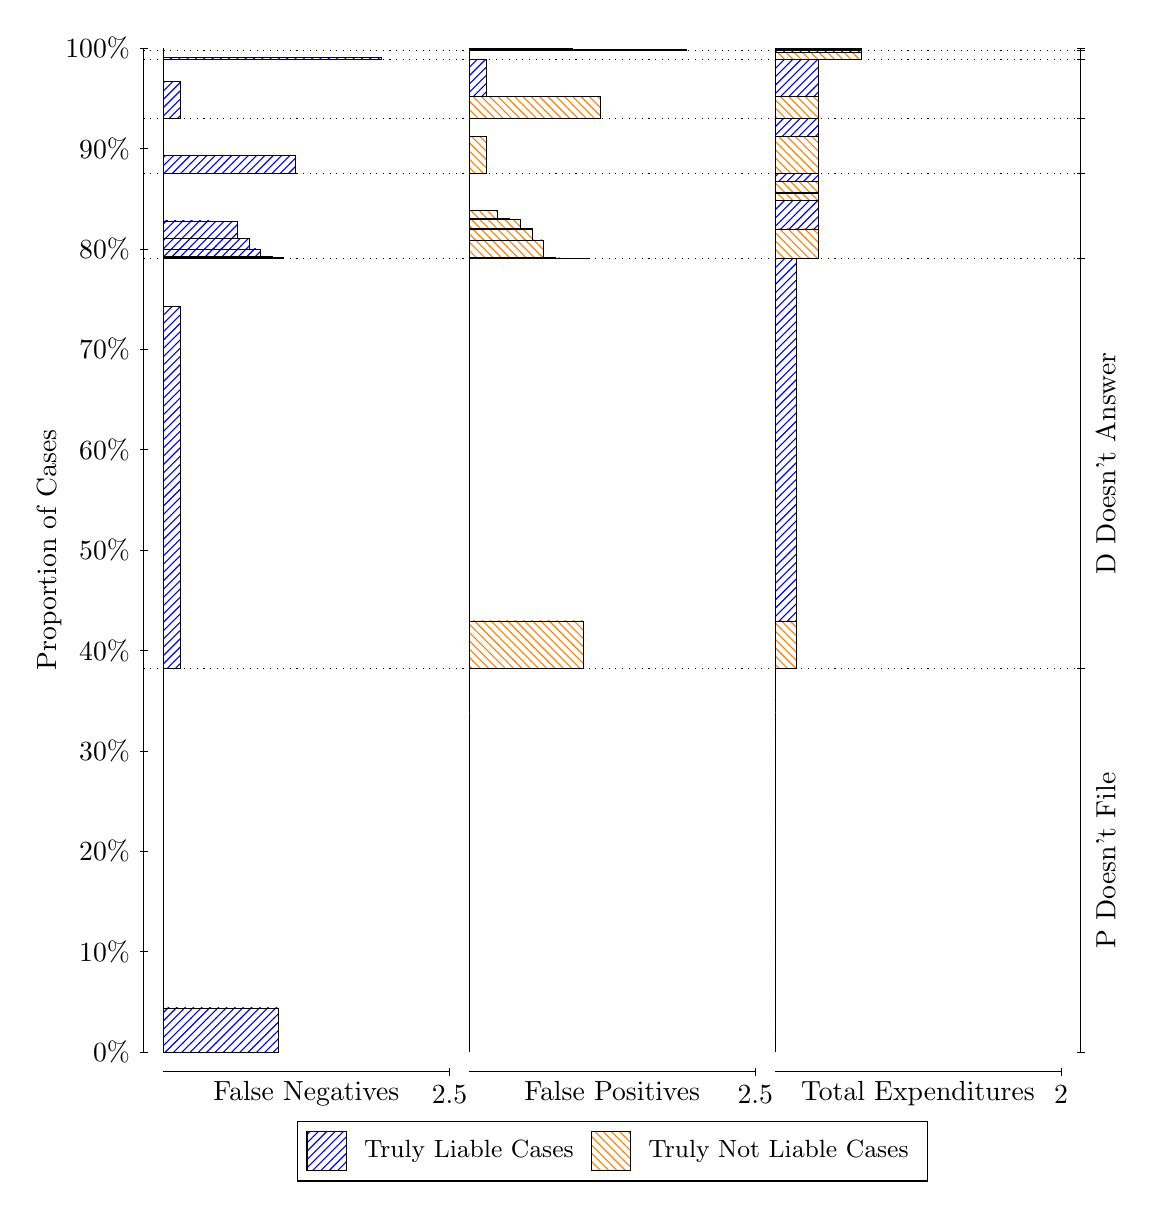
\begin{tikzpicture}
\draw[black, very thin] (1.5,1.75) -- (1.5,14.5);
\node[rotate=90, text=black, anchor=center] at (0.3, 8.125) {Proportion of Cases};
\draw[black, very thin] (1.45,1.75) -- (1.55,1.75);
\node[text=black, anchor=east] at (1.45, 1.75) {0\%};
\draw[black, very thin] (1.45,3.025) -- (1.55,3.025);
\node[text=black, anchor=east] at (1.45, 3.025) {10\%};
\draw[black, very thin] (1.45,4.3) -- (1.55,4.3);
\node[text=black, anchor=east] at (1.45, 4.3) {20\%};
\draw[black, very thin] (1.45,5.575) -- (1.55,5.575);
\node[text=black, anchor=east] at (1.45, 5.575) {30\%};
\draw[black, very thin] (1.45,6.85) -- (1.55,6.85);
\node[text=black, anchor=east] at (1.45, 6.85) {40\%};
\draw[black, very thin] (1.45,8.125) -- (1.55,8.125);
\node[text=black, anchor=east] at (1.45, 8.125) {50\%};
\draw[black, very thin] (1.45,9.4) -- (1.55,9.4);
\node[text=black, anchor=east] at (1.45, 9.4) {60\%};
\draw[black, very thin] (1.45,10.675) -- (1.55,10.675);
\node[text=black, anchor=east] at (1.45, 10.675) {70\%};
\draw[black, very thin] (1.45,11.95) -- (1.55,11.95);
\node[text=black, anchor=east] at (1.45, 11.95) {80\%};
\draw[black, very thin] (1.45,13.225) -- (1.55,13.225);
\node[text=black, anchor=east] at (1.45, 13.225) {90\%};
\draw[black, very thin] (1.45,14.5) -- (1.55,14.5);
\node[text=black, anchor=east] at (1.45, 14.5) {100\%};

\draw[black, very thin] (13.4,1.75) -- (13.4,14.5);
\draw[black, very thin] (13.35,1.75) -- (13.45,1.75);
\node[anchor=west] at (13.35, 1.75) {};
\draw[black, very thin] (13.35,6.6181) -- (13.45,6.6181);
\node[anchor=west] at (13.35, 6.6181) {};
\draw[black, very thin] (13.35,11.828) -- (13.45,11.828);
\node[anchor=west] at (13.35, 11.828) {};
\draw[black, very thin] (13.35,12.911) -- (13.45,12.911);
\node[anchor=west] at (13.35, 12.911) {};
\draw[black, very thin] (13.35,13.608) -- (13.45,13.608);
\node[anchor=west] at (13.35, 13.608) {};
\draw[black, very thin] (13.35,14.355) -- (13.45,14.355);
\node[anchor=west] at (13.35, 14.355) {};
\draw[black, very thin] (13.35,14.472) -- (13.45,14.472);
\node[anchor=west] at (13.35, 14.472) {};
\draw[black, very thin] (13.35,14.5) -- (13.45,14.5);
\node[anchor=west] at (13.35, 14.5) {};

\draw[black, very thin, pattern color=blue, pattern=north east lines] (1.75,1.75) rectangle (3.2033,2.3096);
\draw[black, very thin, pattern color=orange, pattern=north west lines] (1.75,2.3096) rectangle (1.75,6.6181);
\draw[black, very thin, pattern color=blue, pattern=north east lines] (1.75,6.6181) rectangle (1.968,11.22);
\draw[black, very thin, pattern color=orange, pattern=north west lines] (1.75,11.22) rectangle (1.75,11.828);
\draw[black, very thin, pattern color=blue, pattern=north east lines] (1.75,11.828) rectangle (3.276,11.843);
\draw[black, very thin, pattern color=blue, pattern=north east lines] (1.75,11.843) rectangle (3.1307,11.849);
\draw[black, very thin, pattern color=blue, pattern=north east lines] (1.75,11.849) rectangle (2.9853,11.948);
\draw[black, very thin, pattern color=blue, pattern=north east lines] (1.75,11.948) rectangle (2.84,12.084);
\draw[black, very thin, pattern color=blue, pattern=north east lines] (1.75,12.084) rectangle (2.6947,12.298);
\draw[black, very thin, pattern color=blue, pattern=north east lines] (1.75,12.298) rectangle (2.5493,12.302);
\draw[black, very thin, pattern color=blue, pattern=north east lines] (1.75,12.302) rectangle (2.404,12.304);
\draw[black, very thin, pattern color=blue, pattern=north east lines] (1.75,12.304) rectangle (2.2587,12.304);
\draw[black, very thin, pattern color=blue, pattern=north east lines] (1.75,12.304) rectangle (2.1133,12.305);
\draw[black, very thin, pattern color=orange, pattern=north west lines] (1.75,12.305) rectangle (1.75,12.911);
\draw[black, very thin, pattern color=blue, pattern=north east lines] (1.75,12.911) rectangle (3.4213,13.137);
\draw[black, very thin, pattern color=orange, pattern=north west lines] (1.75,13.137) rectangle (1.75,13.608);
\draw[black, very thin, pattern color=blue, pattern=north east lines] (1.75,13.608) rectangle (1.968,14.08);
\draw[black, very thin, pattern color=orange, pattern=north west lines] (1.75,14.08) rectangle (1.75,14.355);
\draw[black, very thin, pattern color=blue, pattern=north east lines] (1.75,14.355) rectangle (4.5113,14.379);
\draw[black, very thin, pattern color=orange, pattern=north west lines] (1.75,14.379) rectangle (1.75,14.472);
\draw[black, very thin, pattern color=orange, pattern=north west lines] (1.75,14.472) rectangle (1.75,14.486);
\draw[black, very thin, pattern color=blue, pattern=north east lines] (1.75,14.486) rectangle (1.75,14.5);
\draw[black, very thin, pattern color=orange, pattern=north west lines] (5.6333,1.75) rectangle (5.6333,6.0585);
\draw[black, very thin, pattern color=blue, pattern=north east lines] (5.6333,6.0585) rectangle (5.6333,6.6181);
\draw[black, very thin, pattern color=orange, pattern=north west lines] (5.6333,6.6181) rectangle (7.0867,7.2257);
\draw[black, very thin, pattern color=blue, pattern=north east lines] (5.6333,7.2257) rectangle (5.6333,11.828);
\draw[black, very thin, pattern color=orange, pattern=north west lines] (5.6333,11.828) rectangle (7.1593,11.829);
\draw[black, very thin, pattern color=orange, pattern=north west lines] (5.6333,11.829) rectangle (7.014,11.83);
\draw[black, very thin, pattern color=orange, pattern=north west lines] (5.6333,11.83) rectangle (6.8687,11.835);
\draw[black, very thin, pattern color=orange, pattern=north west lines] (5.6333,11.835) rectangle (6.7233,11.843);
\draw[black, very thin, pattern color=orange, pattern=north west lines] (5.6333,11.843) rectangle (6.578,12.064);
\draw[black, very thin, pattern color=orange, pattern=north west lines] (5.6333,12.064) rectangle (6.4327,12.204);
\draw[black, very thin, pattern color=orange, pattern=north west lines] (5.6333,12.204) rectangle (6.4327,12.205);
\draw[black, very thin, pattern color=orange, pattern=north west lines] (5.6333,12.205) rectangle (6.2873,12.324);
\draw[black, very thin, pattern color=orange, pattern=north west lines] (5.6333,12.324) rectangle (6.142,12.339);
\draw[black, very thin, pattern color=orange, pattern=north west lines] (5.6333,12.339) rectangle (5.9967,12.434);
\draw[black, very thin, pattern color=blue, pattern=north east lines] (5.6333,12.434) rectangle (5.706,12.434);
\draw[black, very thin, pattern color=blue, pattern=north east lines] (5.6333,12.434) rectangle (5.6333,12.911);
\draw[black, very thin, pattern color=orange, pattern=north west lines] (5.6333,12.911) rectangle (5.8513,13.382);
\draw[black, very thin, pattern color=blue, pattern=north east lines] (5.6333,13.382) rectangle (5.6333,13.608);
\draw[black, very thin, pattern color=orange, pattern=north west lines] (5.6333,13.608) rectangle (7.3047,13.883);
\draw[black, very thin, pattern color=blue, pattern=north east lines] (5.6333,13.883) rectangle (5.8513,14.355);
\draw[black, very thin, pattern color=orange, pattern=north west lines] (5.6333,14.355) rectangle (5.6333,14.448);
\draw[black, very thin, pattern color=blue, pattern=north east lines] (5.6333,14.448) rectangle (5.6333,14.472);
\draw[black, very thin, pattern color=orange, pattern=north west lines] (5.6333,14.472) rectangle (8.3947,14.486);
\draw[black, very thin, pattern color=blue, pattern=north east lines] (5.6333,14.486) rectangle (6.9413,14.5);
\draw[black, very thin, pattern color=orange, pattern=north west lines] (9.5167,1.75) rectangle (9.5167,6.0585);
\draw[black, very thin, pattern color=blue, pattern=north east lines] (9.5167,6.0585) rectangle (9.5167,6.6181);
\draw[black, very thin, pattern color=orange, pattern=north west lines] (9.5167,6.6181) rectangle (9.7892,7.2257);
\draw[black, very thin, pattern color=blue, pattern=north east lines] (9.5167,7.2257) rectangle (9.7892,11.828);
\draw[black, very thin, pattern color=orange, pattern=north west lines] (9.5167,11.828) rectangle (10.062,12.204);
\draw[black, very thin, pattern color=blue, pattern=north east lines] (9.5167,12.204) rectangle (10.062,12.561);
\draw[black, very thin, pattern color=orange, pattern=north west lines] (9.5167,12.561) rectangle (10.062,12.655);
\draw[black, very thin, pattern color=blue, pattern=north east lines] (9.5167,12.655) rectangle (10.062,12.67);
\draw[black, very thin, pattern color=orange, pattern=north west lines] (9.5167,12.67) rectangle (10.062,12.806);
\draw[black, very thin, pattern color=blue, pattern=north east lines] (9.5167,12.806) rectangle (10.062,12.911);
\draw[black, very thin, pattern color=orange, pattern=north west lines] (9.5167,12.911) rectangle (10.062,13.382);
\draw[black, very thin, pattern color=blue, pattern=north east lines] (9.5167,13.382) rectangle (10.062,13.608);
\draw[black, very thin, pattern color=orange, pattern=north west lines] (9.5167,13.608) rectangle (10.062,13.883);
\draw[black, very thin, pattern color=blue, pattern=north east lines] (9.5167,13.883) rectangle (10.062,14.355);
\draw[black, very thin, pattern color=orange, pattern=north west lines] (9.5167,14.355) rectangle (10.607,14.448);
\draw[black, very thin, pattern color=blue, pattern=north east lines] (9.5167,14.448) rectangle (10.607,14.472);
\draw[black, very thin, pattern color=orange, pattern=north west lines] (9.5167,14.472) rectangle (10.607,14.486);
\draw[black, very thin, pattern color=blue, pattern=north east lines] (9.5167,14.486) rectangle (10.607,14.5);
\draw[black, dotted] (1.5,6.6181) -- (13.4,6.6181);
\draw[black, dotted] (1.5,11.828) -- (13.4,11.828);
\draw[black, dotted] (1.5,12.911) -- (13.4,12.911);
\draw[black, dotted] (1.5,13.608) -- (13.4,13.608);
\draw[black, dotted] (1.5,14.355) -- (13.4,14.355);
\draw[black, dotted] (1.5,14.472) -- (13.4,14.472);
\draw[black, very thin] (1.75,1.5) -- (5.3833,1.5);
\node[text=black, anchor=north] at (3.5667, 1.5) {False Negatives};
\draw[black, very thin] (5.3833,1.45) -- (5.3833,1.55);
\node[text=black, anchor=north] at (5.3833, 1.45) {2.5};

\draw[black, very thin] (5.6333,1.5) -- (9.2667,1.5);
\node[text=black, anchor=north] at (7.45, 1.5) {False Positives};
\draw[black, very thin] (9.2667,1.45) -- (9.2667,1.55);
\node[text=black, anchor=north] at (9.2667, 1.45) {2.5};

\draw[black, very thin] (9.5167,1.5) -- (13.15,1.5);
\node[text=black, anchor=north] at (11.333, 1.5) {Total Expenditures};
\draw[black, very thin] (13.15,1.45) -- (13.15,1.55);
\node[text=black, anchor=north] at (13.15, 1.45) {2};

\node[text=black, centered, rotate=90] at (13.72, 4.184) {P Doesn't File};
\node[text=black, centered, rotate=90] at (13.72, 9.2231) {D Doesn't Answer};






\draw (7.449999999999999,1.5) node[draw=none] (baseCoordinate) {};
\begin{scope}[align=center]
        \matrix[scale=0.5, draw=black, below=0.5cm of baseCoordinate, nodes={draw}, column sep=0.1cm]{
            \node[rectangle, draw, minimum width=0.5cm, minimum height=0.5cm, pattern color=blue, pattern=north east lines] {}; &
            \node[draw=none, font=\small, text=black] (B) {Truly Liable Cases}; &
            \node[rectangle, draw, minimum width=0.5cm, minimum height=0.5cm, pattern color=orange, pattern=north west lines] {}; &
            \node[draw=none, font=\small, text=black] (B) {Truly Not Liable Cases}; \\
            };
\end{scope}

\end{tikzpicture}
\end{document}